%*************************************
% ภาคผนวก ข.
%*************************************
\appendixChapterTitle{ข}{การเพิ่มไฟล์ภาคผนวก}
\section{การเพิ่มไฟล์ภาคผนวก}
\hspace*{1.5em}
ตัวอย่างการเพิ่มไฟล์ภาคผนวก เมื่อต้องการเพิ่มภาคผนวก ค. มีรายละเอียดดังนี้
\vspace{0.5em}

\begin{mycustomenum2}
    \item คลิกที่ icon \enquote{New file} ที่มุมบนซ้าย จากนั้นให้ตั้งชื่อไฟล์ ดังภาพที่  \ref{figB:CreateFile1}

\begin{figure}[htbp]
\centering
\adjustbox{frame, width=0.8\textwidth}{
    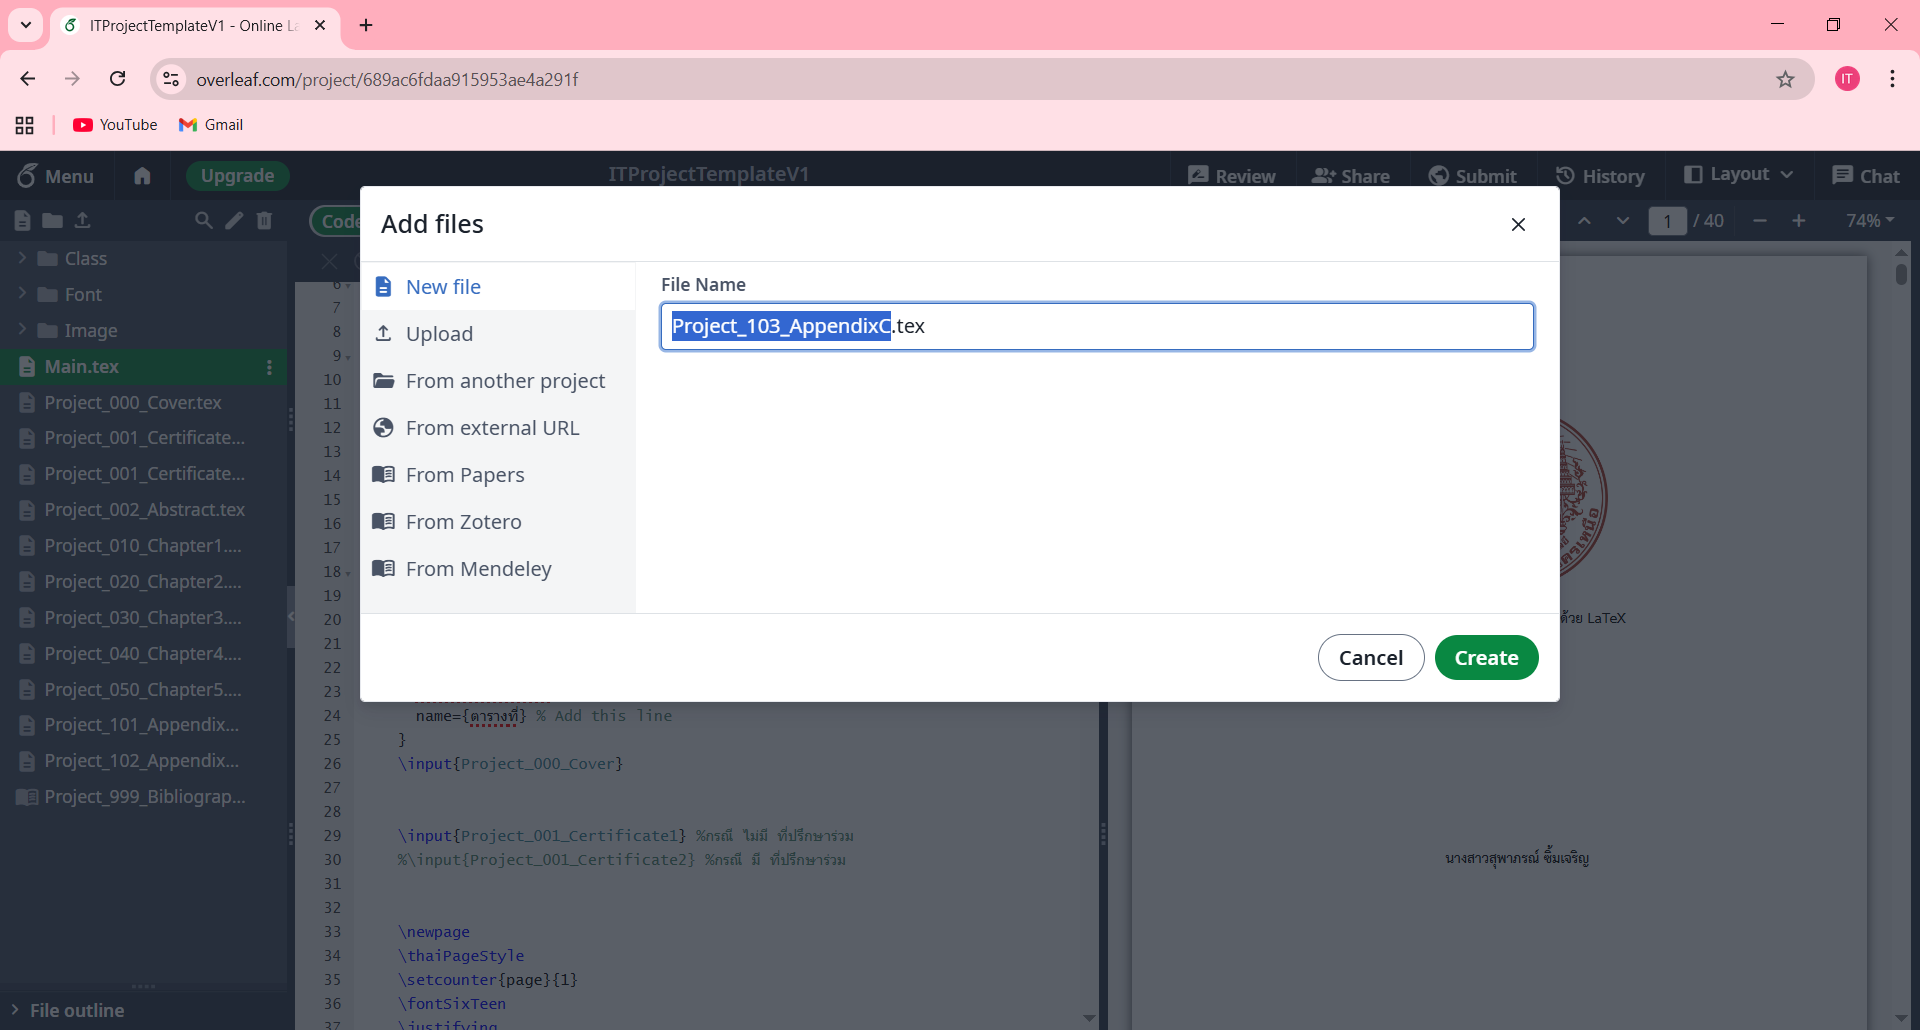
\includegraphics[width=0.8\textwidth]{Image/CreateFile-1.png}
}
\caption{\fontSixTeen{ตั้งชื่อไฟล์ .tex}}
\label{figB:CreateFile1}
\end{figure}

    \item เมื่อคลิกที่ \enquote{Create} ก็สามารถเพิ่มเนื้อหาของภาคผนวก ค. ลงไปได้เลย ดังภาพที่ \ref{figB:CreateFile2}

\begin{figure}[htbp]
\centering
\adjustbox{frame, width=0.8\textwidth}{
    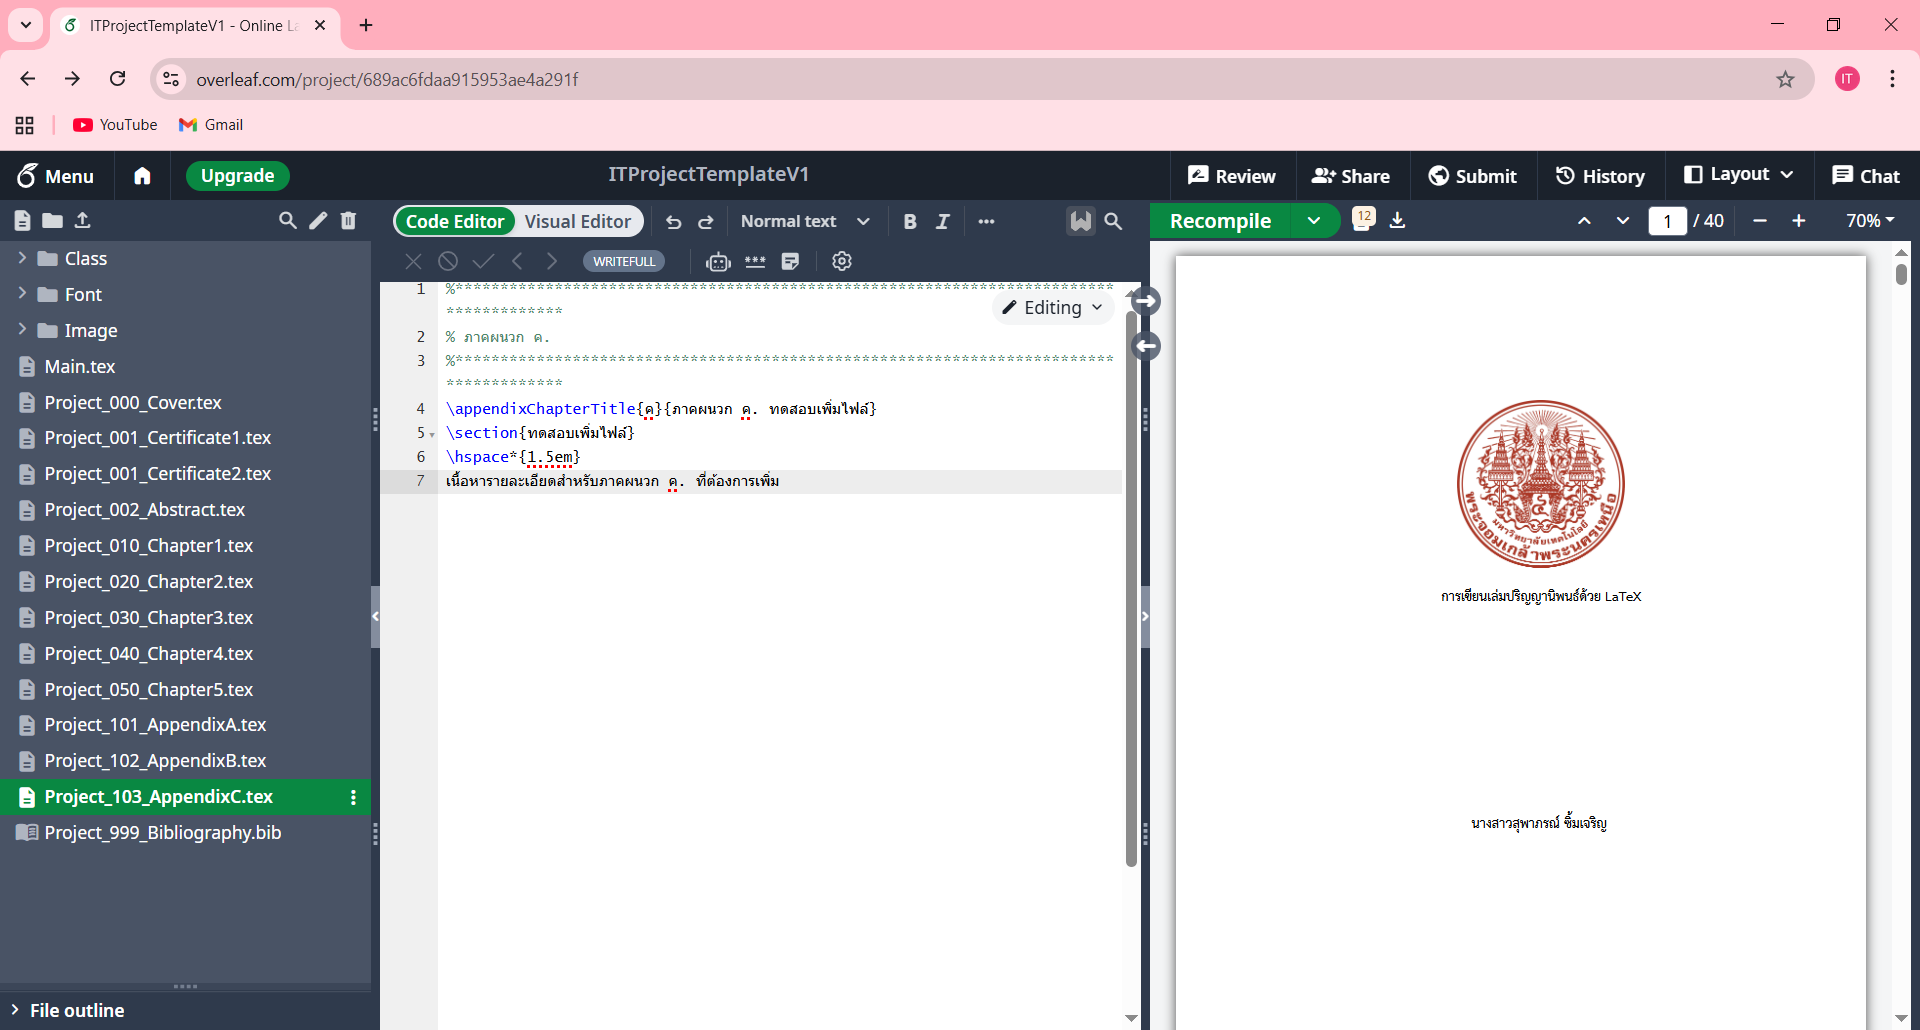
\includegraphics[width=0.8\textwidth]{Image/CreateFile-2.png}
}
\caption{\fontSixTeen{เพิ่มเนื้อหาลงไปในไฟล์ .tex}}
\label{figB:CreateFile2}
\end{figure}

    \item จากนั้นให้ไปเพิ่มโค้ดการเรียกไฟล์ใหม่ที่สร้างขึ้น ที่ไฟล์ Main.tex ดังภาพที่ \ref{figB:CreateFile3}

\begin{figure}[htbp]
\centering
\adjustbox{frame, width=0.8\textwidth}{
    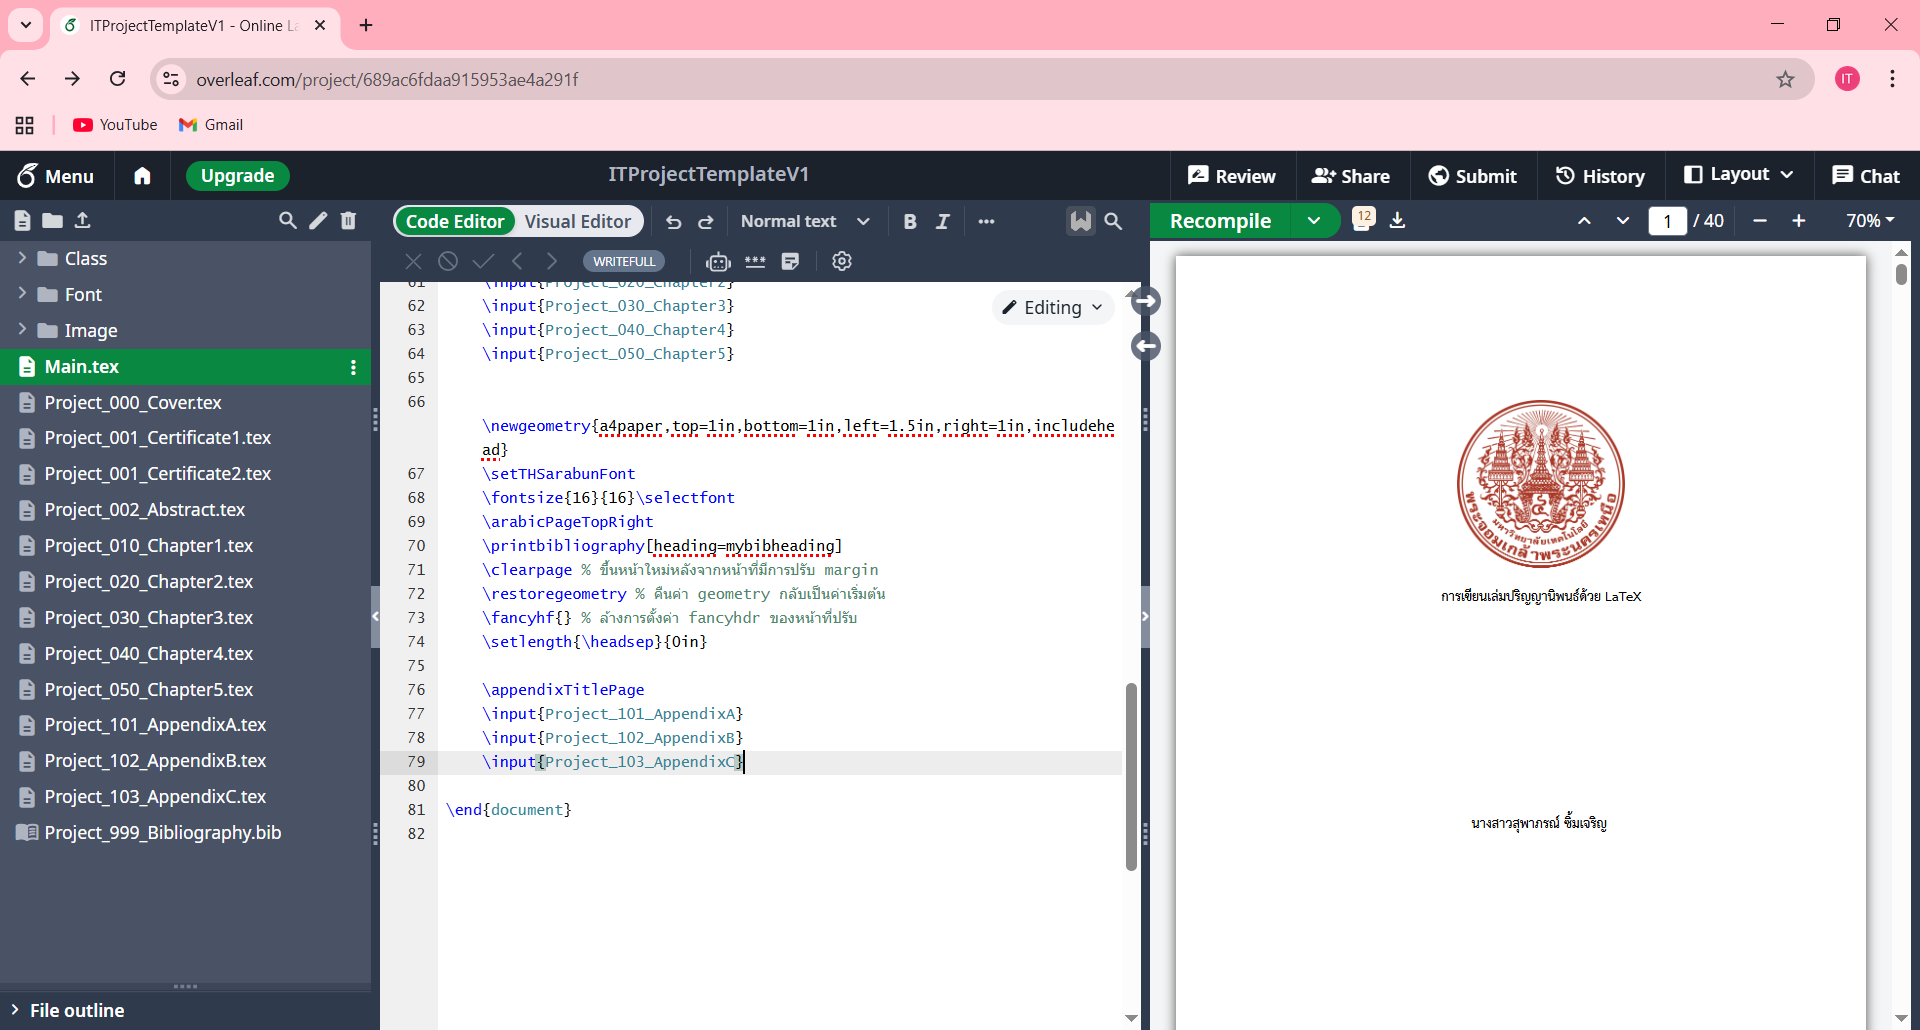
\includegraphics[width=0.8\textwidth]{Image/CreateFile-3.png}
}
\caption{\fontSixTeen{เพิ่มโค้ดสำหรับเรียกไฟล์ .tex ที่สร้างใหม่}}
\label{figB:CreateFile3}
\end{figure}

    \item จากนั้นคลิกที่ Recompile ภาคผนวก ค. ก็จะสามารถใช้งานได้ ดังภาพที่ \ref{figB:CreateFile4}

\begin{figure}[htbp]
\centering
\adjustbox{frame, width=0.8\textwidth}{
    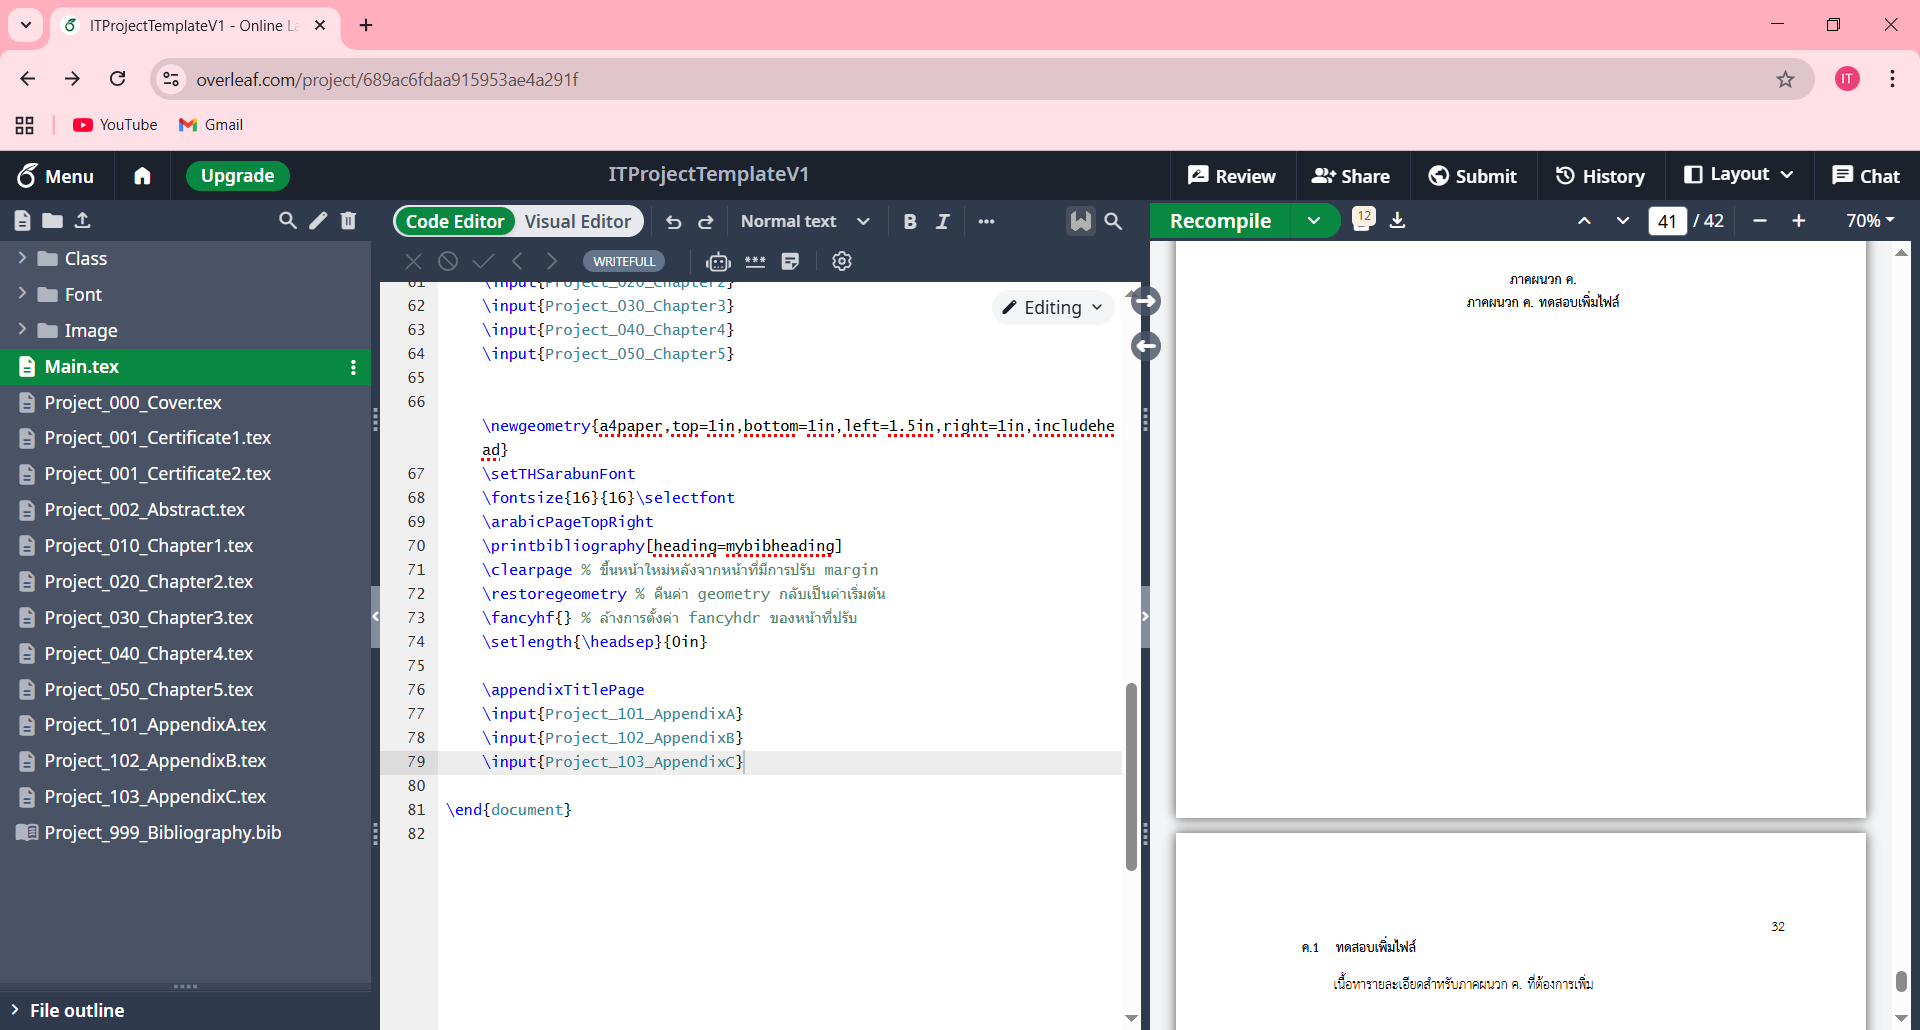
\includegraphics[width=0.8\textwidth]{Image/CreateFile-4.png}
}
\caption{\fontSixTeen{ภาคผนวก ค. แสดงหลังจาก Recompile}}
\label{figB:CreateFile4}
\end{figure}

    \item ในกรณีที่ไม่ต้องการให้เนื้อหาของไฟล์ใดปรากฏ ก็สามารถ Comment ที่โค้ดบรรทัดของการเรียกไฟล์ได้ที่ไฟล์ Main.tex ตัวอย่างการ Comment แสดงได้ดังภาพที่ \ref{figB:CreateFile5} 

\begin{figure}[htbp]
\centering
\adjustbox{frame, width=0.8\textwidth}{
    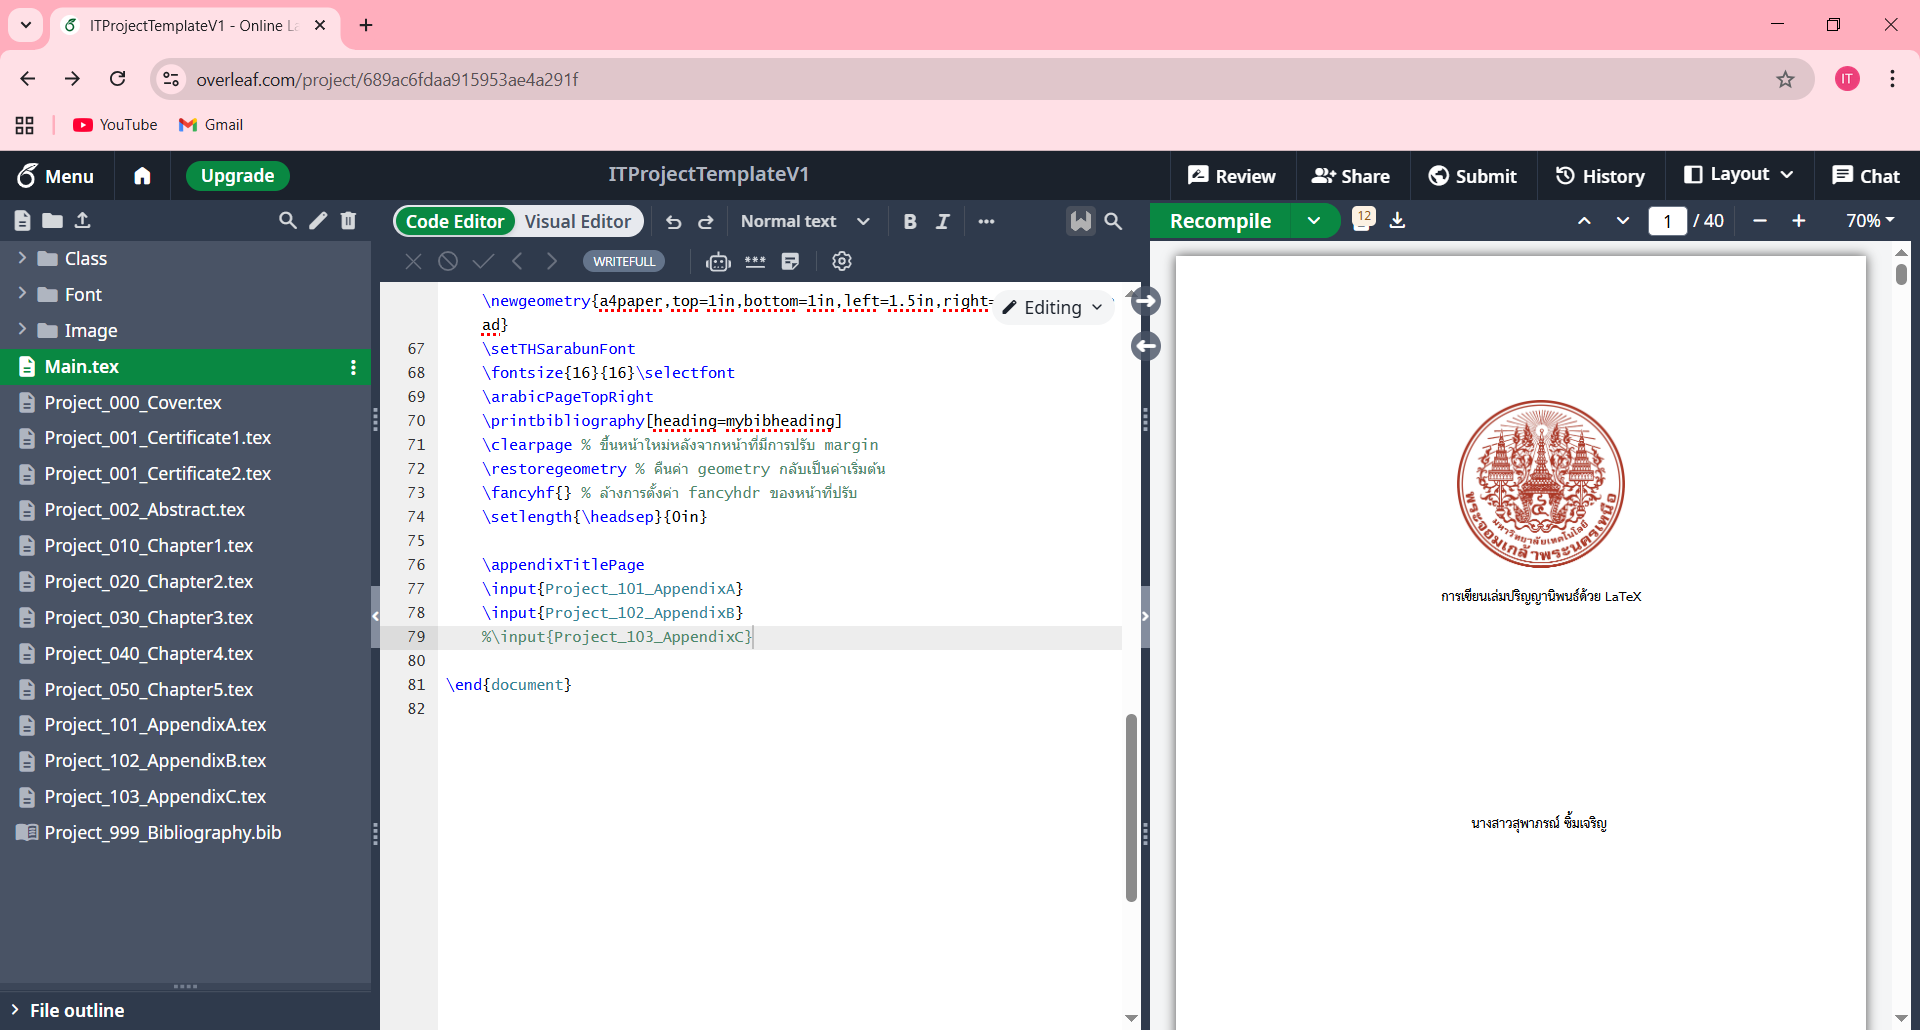
\includegraphics[width=0.8\textwidth]{Image/CreateFile-5.png}
}
\caption{\fontSixTeen{ตัวอย่างการ Comment ไฟล์ .tex ที่ไม่ต้องการแสดง}}
\label{figB:CreateFile5}
\end{figure}

\end{mycustomenum2}